\subsection{Motivation}
Previous experiments on CG applications conducted over cellular networks provided foundational datasets for detecting anomalies related to QoE degradation in CG sessions. However, these datasets were not suitable for performing root cause analysis, as the underlying causes of the anomalies could not be identified. This limitation stemmed from the complex and intrinsic phenomena occurring in real cellular networks, which make it challenging to isolate and attribute specific causes to each observed anomaly. Additionally, while cloud gaming is a significant low-latency application for network operators such as Orange, it primarily serves individual clients. In contrast, industry clients, who represent a major segment of the market, are more likely to leverage CloudVR for their business needs.

Given this context, we chose to focus our data collection efforts on CloudVR applications over Wi-Fi networks. This approach allows us to generate datasets that are specifically designed to facilitate root cause analysis for CloudVR performance issues. Wi-Fi networks offer the advantage of replicating real-world scenarios in controlled laboratory environments. Using Faraday cages, we can emulate various network impairments, enabling us to systematically label the collected datasets for ML training and analysis.

\subsection{Methodology}

In this section, we outline the testbed developed for CloudVR experiments, which leverages the NVIDIA CloudXR architecture to deliver immersive virtual reality experiences over wireless networks. We begin by providing an overview of the CloudVR application framework, followed by a detailed description of the testbed infrastructure and automation components.


\subsubsection{Testbed Infrastructure}

The testbed is built upon the NVIDIA CloudXR SDK, an \ac{XR} streaming platform that utilizes edge computing and cloud-based GPU acceleration to deliver high-fidelity VR experiences. The CloudXR platform streams OpenVR-based applications from a remote server to XR client devices with limited graphical capabilities, such as the untethered \ac{HMDs} Meta Quest 2 and Meta Quest 3. These devices connect to the server through various network interfaces, including Ethernet, Wi-Fi, or cellular connections.

The CloudXR architecture consists of the following key components:;
\begin{itemize}
    \item CloudXR Driver: This server-side driver streams audio and video content from XR applications (e.g., SteamVR) to the client device using network protocols like UDP. 
    \item CloudXR Client: The client-side software enables the HMD to receive and render the streamed VR content while maintaining low latency and high-quality visuals.
\end{itemize}

The CloudVR testbed infrastructure, illustrated in Fig. \ref{fig:chap_2:cloud_xr}, is designed to facilitate controlled experiments under realistic network conditions. It consists of i) a server, a high-performance machine equipped with an Intel(R) Xeon(R) W2235 CPU @ 3.8GHz with 32 GB of RAM, NVIDIA GeForce RTX 3090 Ti with 24GB,, running the CloudXR server software to render and stream VR content; ii) a thin client, the Meta Quest 2 HMD, which acts as the client device, connected wirelessly to the network and iii) a Wi-Fi \ac{AP}, a Orange commercial Livebox router that serves as the wireless bridge between the server and the HMD.

\begin{figure*}[!t]
    \centering
    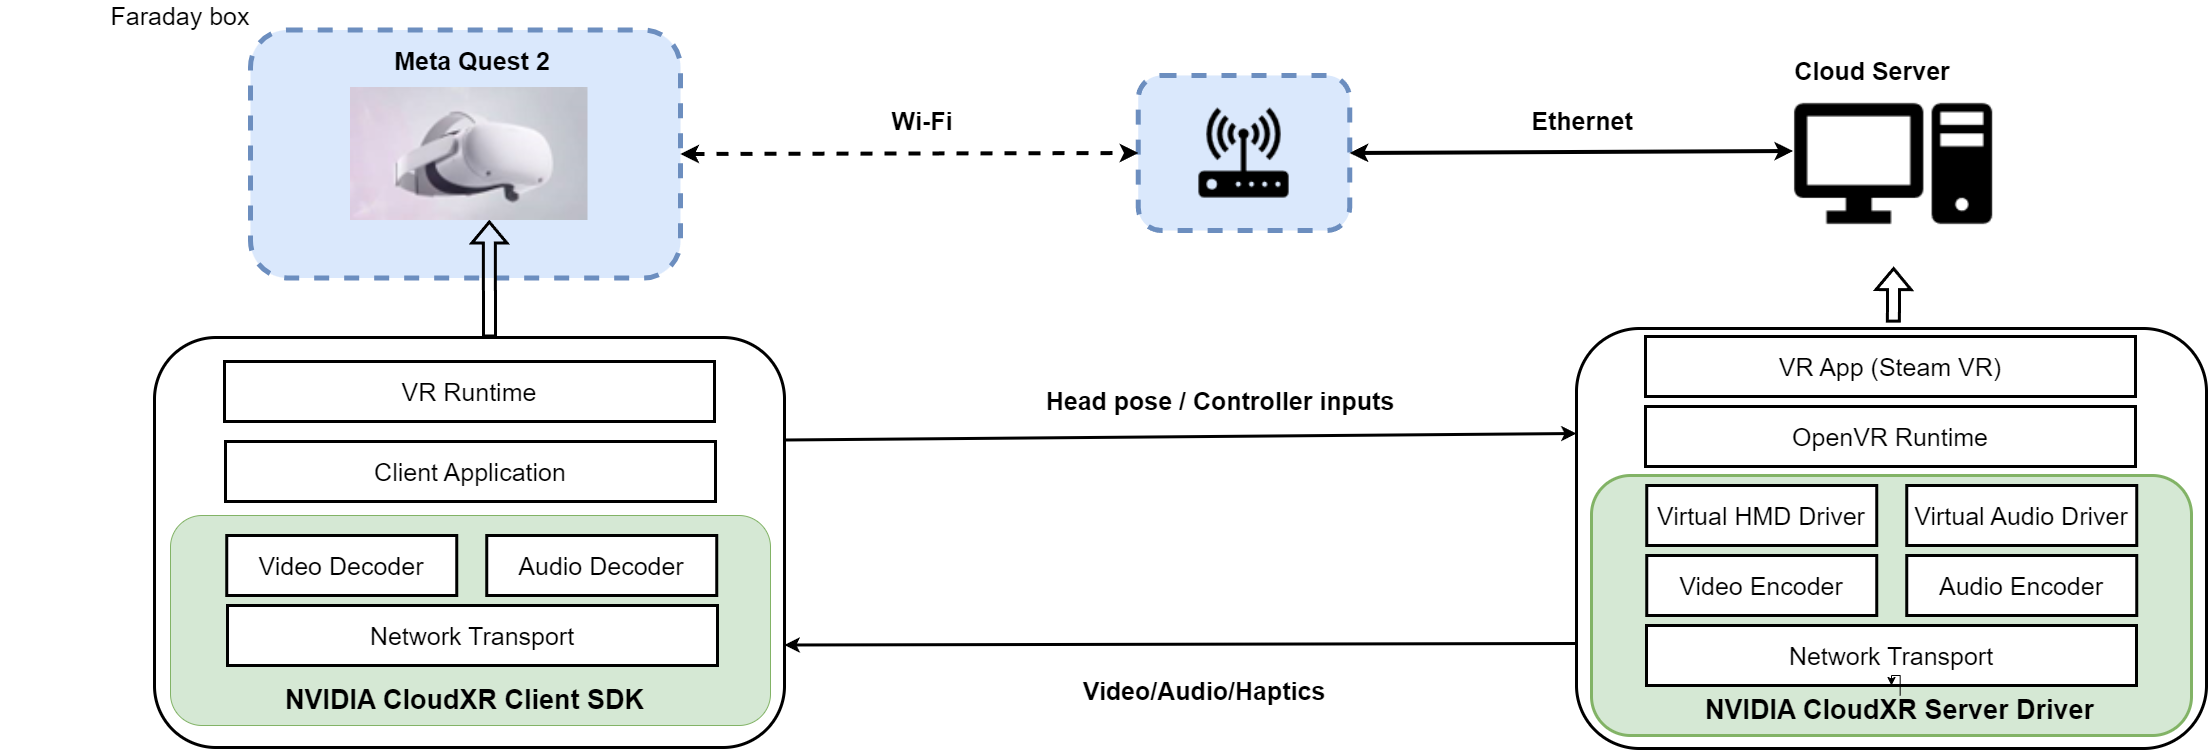
\includegraphics[width=\linewidth]{imgs/chapter_2/cloud_xr_stack.png}
    \caption{Cloud XR Architecture}
    \label{fig:chap_2:cloud_xr}
\end{figure*}


\subsubsection{Wi-Fi Testbed for Controlled Experiments}

Wi-Fi networks are critical for ensuring seamless connectivity for CloudVR applications, but they are inherently susceptible to performance degradation due to obstacles, interference, and competing traffic. To study these challenges systematically, we designed a controlled Wi-Fi testbed, as illustrated in Fig. \ref{fig:chap_2:wifi_testbed}. This setup allows for the reproduction of real-world scenarios and controlled network impairments in laboratory conditions, enabling detailed analysis of their impact on CloudVR services.

The testbed consists of two primary layers:
\begin{itemize}
    \item \textbf{Infrastructure layer:} This layer includes up to four Faraday cages used to isolate equipment from external electromagnetic interference. The cages are allocated as follows: one for the VR headset, two for the APs, and one for a station used in interference scenarios. The layer also includes two access points (AP1 and AP2): AP1 is utilized for normal and coverage experiments, while AP2 introduces interference in specific scenarios. The Faraday cages are interconnected using coaxial cables to transmit Wi-Fi signals, and \ac{RF} attenuators \footnote{\url{https://adauratech.com/attenuators/}} are employed to simulate variations in signal strength during experiments. Two servers are part of this setup: the first server (see Fig. \ref{fig:chap_2:cloud_xr}) runs the CloudVR software and is connected to AP1 via Ethernet, while the second server acts as a traffic generator connected to AP2, simulating competing downlink traffic using UDP.

    \item \textbf{Control and Automation layer:} This layer includes a VR PC controller connected to the VR headset via USB, responsible for managing headset settings and collecting performance metrics, such as KPIs from OVR Metrics tools\footnote{\url{https://developers.meta.com/horizon/downloads/package/ovr-metrics-tool/}} or quality-of-service (QoS) statistics from CloudXR. The controller also automates game sessions using the Meta Quest Autodriver\footnote{\url{https://developers.meta.com/horizon/documentation/unity/ts-autodriver}}. Additionally, this layer features an attenuator controller that configures and manages RF attenuators via APIs, enabling automated signal attenuation adjustments through FastAPI \footnote{\url{https://fastapi.tiangolo.com/}}. Furthermore, the Livebox controller manages the Livebox via Telnet to collect Wi-Fi KPIs every 3 seconds. A local ELK Stack \footnote{\url{https://www.elastic.co/fr/elastic-stack}} database aggregates data from all controllers for post-experiment analysis.

\end{itemize}

\begin{figure*}[!t]
    \centering
    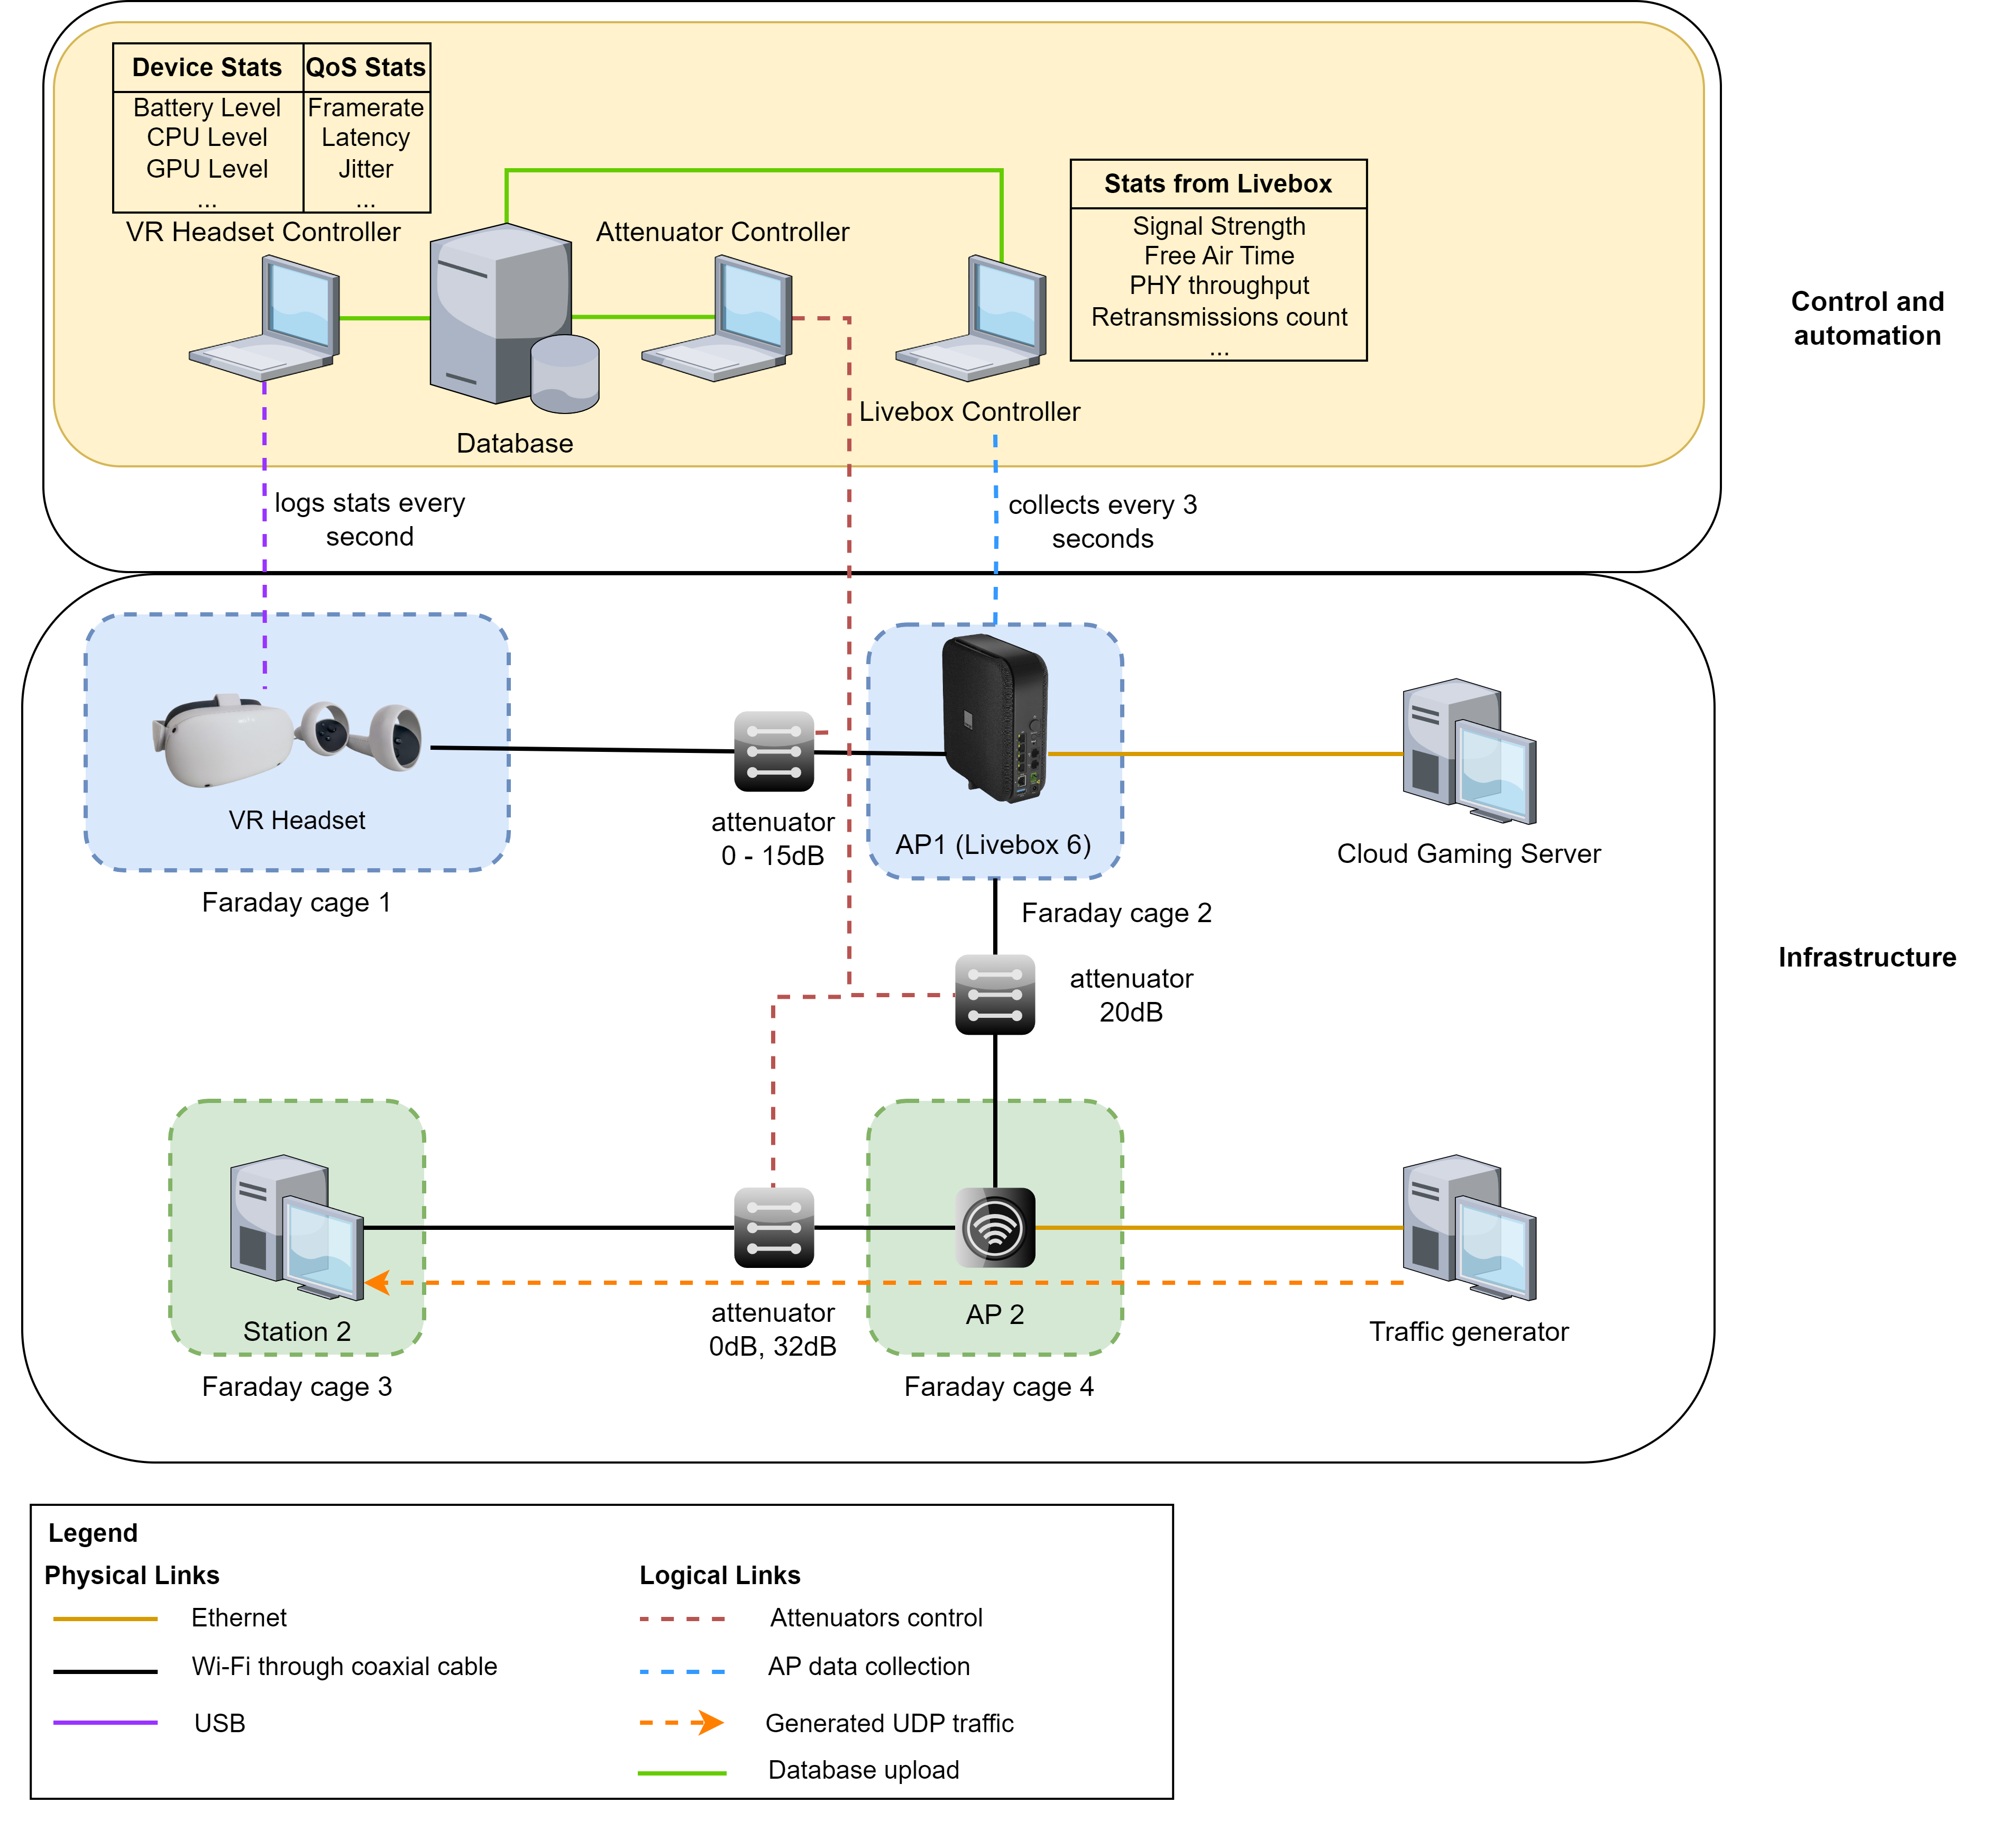
\includegraphics[width=\linewidth]{imgs/chapter_2/WiFi_testbed.png}
    \caption{Wi-Fi testbed architecture}
    \label{fig:chap_2:wifi_testbed}
\end{figure*}

\subsubsection{Scenarios considered}

We collect Cloud VR data across several controlled scenarios using the Beat Saber game as a benchmark. These scenarios were executed on both the 2.4 GHz and 5 GHz frequency bands, as detailed below:
\begin{itemize}
    \item \textbf{Normal scenarios :} CloudVR sessions were conducted under ideal conditions, without any Wi-Fi impairments. The VR headset was positioned in an optimal coverage area and connected to the primary access point (AP1) for each frequency band. A total of 5 sessions, each lasting 300 seconds, were performed for both the 2.4 GHz and 5 GHz bands.
    \item \textbf{Coverage scenarios :} To evaluate the impact of signal strength variations, an RF attenuator was used to simulate different received signal strength indicator (RSSI) values during VR sessions agter launching the game. RSSI levels of \{-55 dB, -60 dB, and -65 dB\} in 2.4 GHz and RSSI levels of \{-80 dB, -85 dB, and -90 dB\} in 5GHz. Each configuration was tested in three sessions, with each session lasting 100 seconds.

    \item \textbf{Interference scenarios :} Interference was introduced by a neighboring station connected to a secondary access point (AP2) operating on the same frequency and bandwidth as AP1. The interference was simulated by occupying a portion of the transmission opportunities (txops) available on AP1 after starting the game. Interference levels leaving \{10\% and 15\%\} of txops in 2.4 GHz band and interference levels leaving \{9\%, 10\%, and 11\%\} of txops in 5GHz for AP1. Each configuration was tested in three sessions, with each session lasting 100 seconds.
\end{itemize}

The testbed configuration ensures a highly controlled environment for Cloud VR experiments. By utilizing Faraday cages, we eliminate uncontrolled radio interference, and by deploying local servers, we remove fluctuations from external network segments. Automation allows for the seamless execution of test scenarios and comprehensive data collection of Cloud VR applications.




\subsubsection{Data collected}

During the Cloud VR experiments, three distinct types of data were collected to comprehensively capture application performance and network behavior:
\begin{itemize}
    \item \textbf{Application-Level Metrics}: Metrics were obtained directly from the Oculus OVR Metrics Tool, which provides detailed insights into the performance of the VR application on the headset. These include frame rates, resolution, CPU and GPU levels and usage, and other statistics related to VR streaming. These metrics help evaluate the QoE from the perspective of the end user. Additionally, QoS metrics were retrieved from the NVIDIA CloudXR stack, which facilitates the streaming of high-quality VR content from the server to the headset. These metrics include network round trip delay, client queuing time, packet loss, and jitter.
   \item \textbf{Livebox-Level Metrics}: The collected Wi-Fi KPIs include metrics from the Wi-Fi physical layer, such as \ac{RSSI}, background noise levels, free airtime, \ac{MCS} index, channel bandwidth, and physical layer bitrates, as well as metrics from the network layer, such as data bitrates, dropped and retried packets, and packet counters for the \ac{BSS}. These metrics were collected directly from the proprietary Livebox router to monitor and evaluate the Wi-Fi conditions experienced during the Cloud VR sessions.
   \item \textbf{Raw Traffic Captures}: \ac{PCAP} data was collected using a probe placed in the Faraday cage near the VR headset. These raw traffic captures provide a detailed view of packet-level interactions between the VR client and the server, including timestamps, protocol usage, packet sizes, and packet inter-arrival times, which may be useful for detecting potential anomalies at the transport and application layers.
\end{itemize}


\usage{For the experiments presented in this work, the \ac{RCD} focused solely on the Livebox-level metrics. These metrics were used to detect and classify anomalies affecting the Wi-Fi performance during Cloud VR sessions. The application-level and raw traffic metrics, while not utilized in the current analysis, present opportunities for future work. They could enhance diagnostic performance by providing richer context and additional data points for identifying the underlying causes of performance degradation.

The datasets will be available as OpenData.}



